\chapter{Generator}

\section{Storage of source data}

The generator of spatio-temporal and textual data uses real point of interests on the map as a source of data. These data where extracted from the online 
travel service TripAdvisor, using an already implemented crawler \cite{25}. These points of interest are identified on the map by their geographical coordinates, as 
well as their address. Also, they come with ratings and reviews by real TripAdvisor users. The number of such available points is 136409, as they were extracted by 
a 13GB response json file from the crawler. The points where stored in PostgreSQL. The database schema used, contains two tables, one for the points of interest 
and one for the reviews and ratings of these points and is the following:

\begin{figure}[H]
  \centering
  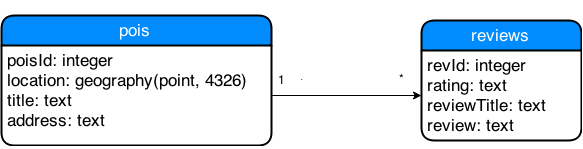
\includegraphics[width=0.7\textwidth]{figures/schema.png}
  \caption{Database schema for source data}
\end{figure}

More specifically, the table for the points of interest has the following attributes:

\begin{itemize}
 \item poisId: identifying number for the point of interest, primary key.
 \item location: geographical coordinates of the point. Usage of the geographic data type introduced by the extension PostGIS of PostgreSQL.
 \item title: the name of the point of interest.
 \item address: the address of the point on the map.
\end{itemize}

A point of interest can have many reviews, issued by different users, thus the two tables are associated by 1-to-many. The reviews table contains 
the following attributes:

\begin{itemize}
 \item revId: the identifying number of the point of interest that the review refers to, foreign key.
 \item rating: rating of the point in a scale of 1 to 5.
 \item reviewTitle: the title of the review.
 \item review: the text of the review.
\end{itemize}

After storing all points of interest into the database, we create an B-tree index to the attribute poisId of the table pois and to the attribute revId of the table reviews, 
as well. Additionally, er create a GiST index to the attibute location of the table pois. As location has a geographic data type, GiST will implement an 
improved R-tree index, as described in section 2.2.2. In this way, searching points of interest accrding to their location or identifying number, can be done 
fast and efficiently.

\section{Generator attributes}

The following class diagram indicates the main attributes used in the description of the generator's design.

\begin{figure}[H]
  \centering
  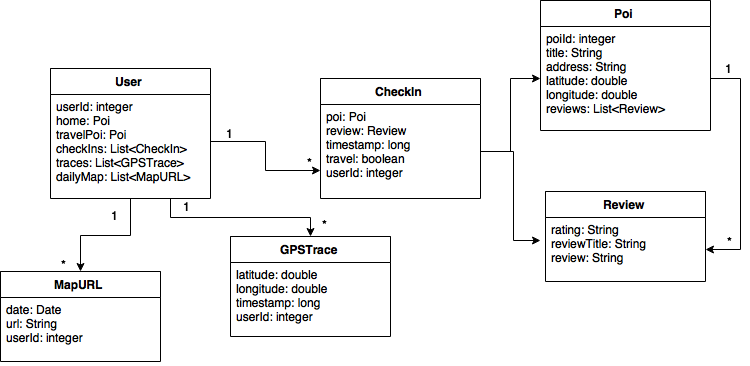
\includegraphics[width=0.9\textwidth]{figures/class_diagram.png}
  \caption{Class diagram of generator's attributes}
\end{figure}

\subsection{User}

The user produced by the generator has the following fields:

\begin{itemize}
 \item userId: user's identifier.
 \item home: user's home defined as Poi.
 \item travelPoi: the central location of the current trip, defined as Poi.
 \item checkIns: list of user's check-ins during the days for which the generator produced data.
 \item traces: list of GPS traces indicating the user's daily routes during the days for which the generator produced data.
 \item dailyMap: list of URLs to static maps images showing the daily user routes.
\end{itemize}

\subsection{Check-in}

A check-in to a point of interest (POI) has the following fields:

\begin{itemize}
 \item poi: the point of interest (Poi) where the check-in was made.
 \item review: the review that the user made for the specfic POI on the check-in.
 \item timestamp: the time when the check-in was made, in representation of type long.
 \item travel: boolean value indicating whether the check-in was made during a user's trip.
 \item userId: the user's identifier.
\end{itemize}

\subsection{GPS trace}

A user's route consists of multiple GPS traces, which illustrate the path that the user followed. A GPS trace contains the following information:

\begin{itemize}
 \item (latitude, longitude): the geographical coordinates of the point on the map where the GPS trace was taken.
 \item timestamp: the time when the GPS trace was taken.
 \item userId: user's identifier whose route contains the specific GPS trace.
\end{itemize}

\subsection{Static route map - MapURL}

A user's daily route is depicted on a static map, using Google Static Maps API. The map shows the points of interest that the user visited using markers, 
and the exact path from one POI to another using blue continuous lines. The image of the map can be accessed through a respective URL.

\begin{itemize}
 \item url: the URL that directs to the image of the map.
 \item date: the date when the user walked the route showed on the map.
 \item userId: the identifier of the user who walked the specific route that date.
\end{itemize}

\subsection{Point of interest - Poi}

A point of interest has the following attributes:

\begin{itemize}
 \item poiId: point's identifier.
 \item title: point's name.
 \item address: point's address.
 \item (latitude, longitude): point's geographical coordinates.
 \item reviews: a list with the available reviews for the specific point.
\end{itemize}

\subsection{Review}

A review to a point of interest has the following fields:

\begin{itemize}
 \item rating: rating of the POI in scale 1 to 5.
 \item reviewTitle: the title of the review.
 \item review: the text of the review.
\end{itemize}

\section{Input parameters}

The generator takes as input the next parameters: 

\begin{itemize}
 \item userIdStart: identifier of the first user for whom the generator will create daily routes.
 \item userIdEnd: Respectively, the identifier of the last user created.
 \item chkNumMean: The mean of the number of daily check-ins to points of interest, which will follow a normal distribution.
 \item chkNumStDev: The standard deviation of the normal distribution that the number of daily check-ins follow.
 \item chkDurMean: The mean of the duration that each visit will last, which will follow a normal distribution.
 \item chkDurStDev: The standard deviation of the normal distribuition of the duration of user's visits.
 \item dist: The maximum distance in meters in which a user can walk from one point of interest to the next one.
 \item maxDist: The maximum distance in meters from a user's home, in which a user can walk every day.
 \item startTime: The time when the first check-in of the day will occur.
 \item endTime: The time when the last check-in of the day will occur.
 \item startDate: The first day starting from which the generator will create daily routes.
 \item endDate: Respectively, the last day that the generator will create daily routes.
 \item outCheckIns: The output file storing the daily check-ins of all users created.
 \item outTraces: The output files storing the GPS traces of the daily routes of all users created.
 \item outMaps: The output file storing the URLs for the daily maps depicting the daily routes of all users created.
\end{itemize}

\section{Generator's implementation design}

The generator's main function is to create user's daily routes, which will contain information simulating real social media data. These daily routes 
consist of visits (check-ins) to points of interest and paths that the user followed from one point to the next one. The generator takes as input the 
values of the corresponding parameters and based on the stored source data, creates daily routes for (userIdEnd - userIdStart + 1) users between 
the start and end dates. The decisions that the generator makes, such as how many points the user will visit a specific day, or the duration 
of each visit, are made using random factors. In this way, the produced data can be as realistic as possible. The generator stores the created data in three files, 
one for all the user check-ins (outCheckIns), one for the all the GPS traces (outTraces) and one for the all the daily maps (outMaps).

\subsection{Home definition}

The location of a user's home is the center around which he walks every day. The points of interest that a user visits are selected in a random way, thus there can 
exist routes that don't make sense. For example, a user can walk one day in Greece, the next day in France and the other day again back in Greece. This is the reason 
why the location of a user's home is specified, so that a user can walk in a sensible distance from his home every day. More specifically, a user can walk in a range 
of maxDist meters from his home, as those are defined by the according input parameter. In the implementation of the generator, the home of a user is defined as 
the point where his first ever visit is made on startDate. The choice of this point is done using a generator of random numbers which follow a uniform distribution. 
The range of the distribution are the total number of source POIs stored in PostgreSQL.

\subsection{Trip definition}

A user created by the generator is capable to travel, so as to be able to visit places that are further than maxDist meters from his home. In this way, 
routes one day in Greece and the next one in France make sense. However, there has to be defined a central point around which the user will walk during his trip. 
In the implementation of the generator, this point is chosen to be the first ever point that the user visits during the current trip. 
The choice of that point is done using a generator of random number that follow a uniform distribution. The range of the distribution is the number 
of available source POIs.

As far as the duration of each trip is concerned, each user can travel for a time interval that equals the 10\% of the total time interval for which the generator 
produces daily routes. The days of the time interval can be spread out to multiple trips. The duration of each trip is defined using a generator of random numbers 
which follow a normal distribution. The mean of this distribution is declared to be 5 and the standard deviation is 2. In this way, according to the 
3-sigma empirical rule for the normal distribution, 95\% of the random trip durations will be between 1 and 9 days, which is reasonable for short and long trips. 
To sum up, if the user is about to travel the next days, the duration of the trip is defined in a random way and if the duration of the trip doesn't exceed the 
available travel days, the prospective trip begins. If the duration of the trip exceeds the available days, then the trip is calculated to last for the 
available days.

Finally, the decision whether the user will begin a trip or not is made in a random way, using a generator of random numbers that follow the Bernoulli distribution. 
Thus, the generator decides every day whether or not to start a trip for the current user. This decision ressembles a fair coin toss. Therefore, 
if the generator decides to start a trip for the current user, then it decides, in a random way as well, the duration and the location of the trip. Each 
daily route during the trip has to be in maxDist range from the trip's central location.









